In order to eliminate the Chainsewing Attack we propose an update to the NIPoPoWs
protocol under velvet fork. The core problem is that in her suffix proof the adversary
is able to claim not only blocks of a forked chain,  which are in majority adversarially
generated due to the Common Prefix property, but also an arbitrarily long part of the
chain adopted by an honest player. Since thorny blocks are accepted as valid,
the verifier cannot distinguish blocks that actually belong in a chain from
blocks that only seem to belong in the same chain because they are pointed to
via a non-smooth pointer. \\

%% first reference to 1/3 adversary
These facts make it possible to provide a secure solution for the velvet fork
conditions only under the assumption of adversary of $1/3$ of the total hashing
power of the updated honest miners. This claim is described and discussed in
the following.

\subsubsection*{Impossibility of a secure protocol for (1/2)-bounded adversary}
During our study on the problem we failed to prove the security of several protocol
constructions under $(\frac{1}{2})$-bounded adversary. We finally concluded that
such a secure NIPoPoWs construction is impossible under velvet fork conditions.
Though it is hard to provide a typical proof for this claim, as one should consider
any possible construction, in this section we will try to argue for it.

\textbf{Claim:} \textit{Assume $t$ adversarial out of total $n$ parties. There is
no construction for NIPoPoWs suffix proofs under velvet fork conditions, which is
secure for every adversary, such that $\dfrac{t}{n-t} < 1 - \delta$.}

\textit{Discussion.} As explained earlier, since the adversary may use the interlink
structure so as to include pointers to arbitrary blocks,  she may construct her own
chain history utilizing the false pointers included in the blocks she herself generates.
Such an example is given in Figure \ref{fig:generic_attack}.

Let us consider a construction $p$ which allows for NIPoPoWs suffix proofs under velvet
fork and is secure for the underlined conditions. In order $p$ to have a chance for
being secure, it should be possible to challenge the submitted proofs, so that an
honest player can contest against an inconsistent proof. Note that the same power
to challenge any submitted proof is also provided to the adversary.

Now assume an adversary of $ \frac{n}{3} < t < \frac{n}{2} $. Then, as explained
in the Backbone and Selfish Mining papers \cite{Backbone}\cite{selfish_mining} it
is possible for the adversary to maintain the longest valid chain being of less
than $50\%$ chain quality in favor of adversarially generated blocks. This is
illustrated in Figure \ref{fig:selfish_mining_pie}.

\begin{figure}[h!]
	\begin{center}
		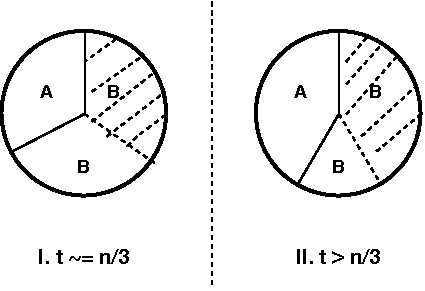
\includegraphics[scale=0.8]{figures/selfish_mining_pie.pdf}
	\end{center}
	\caption{\textit{Pie chart of adversarially and honestly generated blocks distribution
	during a round set S. Part \textbf{A} stands for blocks mined by the adversary while
	\textbf{B} for blocks mined by honest parties. Lined out parts denote honestly mined
	blocks that were defeated by adversarially mined ones in the same round due to selfish
	mining. The rest denote blocks placed in the chain adopted by honest parties.
	\textbf{I.} With $t = n/3$, $50\%$ of the total blocks are adversarially generated
	in the worst case scenario. \textbf{II.} With $t > n/3$, more than half of the
	total blocks are adversarially generated in the worst case scenario.}}
	\label{fig:selfish_mining_pie}
\end{figure}

Observe that the property violated in the described attack is the $prevId$ relation
between sequential blocks. However since the main purpose of our work is to achieve
succinctness, the \textit{prevId} relations could not be utilized in a viable manner
in order to contest adversarial proofs, as it would require proofs of linear length
to that of the whole chain.  We thus conclude that we should mostly rely on the
information given by the interlink data structure as far as the validity of any proof
is concerned so as to keep our protocol construction efficient.

Now assume, to honest parties' favor, that it is both possible and efficient to inspect
the whole chain history that each block is commited to via its interlink pointers. Keep
in mind that an adversary can keep a consistent chain considering the interlink pointers
by using only her own mined blocks and, at the same time, these blocks may overwhelm
the honestly generated ones. In our protocol $p$ it should be decided  under what policy
an honest party generates blocks and constructs suffix proofs. A decision should be made
for block generation:
\begin{enumerate}
\item interlink data are neutral as for adversarially and honestly generated blocks
\item interlink data point out inconsistent blocks, meaning blocks with incorrect
interlinks\item interlink data exclude inconsistent blocks from being part of the
valid chain formed by the super-pointers
\end{enumerate}
Now let's examine the above choices. \\
In the first case the arguments that an honest player could provide against an
inconsistent proof could only be based on the 0-level pointers. Such a contesting
proof should at least provide the 0-level subchain of length equal to the
following: starting from a block included in the suffix proof and is not a
block of the chain until the closest block included in the suffix proof and is
a valid block of the chain. This means that contesting proofs are expected to
be of length $2^\mu$ where $\mu = log(|C|)$, and subsequently are of complexity
$\mathcal{O}(|C|)$ which ruins the succinctness of our protocol.

In the second case an honest party could utilize this extra information provided
in the interlink to prove an inconsistent proof wrong. However, keep in mind that
the adversary could make such claims too. So, a claim of inconsistency for a
specific block included should be followed by a proof of its inconsistency.
Whatever the information considering the incorrect blocks in the interlink may
be, the adversary could make some of it in her own generated blocks in order to
contest an honest proof too. So we fall to the previous case turning to
\textit{prevId} pointers in order to prove the true chain history, where the
contesting proofs are unacceptable efficiency-wise.

In the third case we demand from the honest players to validate the interlink
structures of the blocks in the chain and exclude the inconsistent ones from
the chain history that the interlinks provide. In this way we could possibly
provide contesting proofs using information only from the interlinks thus
keeping our proofs succinct. This solution would result to two different
chain histories considering the interlink pointers: the one of the honest
parties that includes only blocks with valid interlinks, and the one of the
adversary which may form her own history of invalid blocks probably belonging
to many different underlying chains but could not include honest blocks if at
least one invalid block participates in the proof. This solution seems to bring
us to a notable trade-off point. On the one hand we manage to uncouple from the
0-level blocks. On the other hand, we compromise that honest players cannot use
valid adversarially generated blocks in their proof, while the adversary cannot
include honestly generated blocks in her proofs if inconsistent blocks are also
included. This solution could not work properly for $(\frac{1}{2})$-bounded adversary
though. The reason lies in the bad chain quality as pointed out earlier and shown in
Figure \ref{fig:selfish_mining_pie}. If the adversary  could create his own chain
history including inconsistent blocks from two different chains, then she could
easily construct a suffix proof that wins over an honest one because the majority
of the blocks included in the chain could be adversarial with high probability.

We conclude that such a protocol could not exist for $(\frac{1}{2})$-bounded adversary.


\subsubsection*{Solution for (1/3)-bounded adversary}
The vulnerability that makes this attack possible is the acceptance of blocks
containing false interlink pointers. Since we operate under a velvet fork we
cannot eliminate such blocks, but we need, however, to restrict the adversary
from being able to claim portion of another chain as part of her own fork chain.
The key observation on the Chainsewing Attack is that the adversary needs at
least one adversarially generated block in an honest player's chain (block $a'$),
in order to create a path of superpointers connecting blocks of two, or more,
diverse chains. The final proof chain will make use of this crossing point and
may contain both honest or adversarial blocks.
%% intuitive reference to 1/3 adversary
In case the proof contains only adversarial blocks, the attack cannot harm
security for an adversary of less than $1/3$ hashing power. This fact will be
clear in the security proof section. In short, as argued in the previous section
an adversary of $1/3$ of the total hashing power may contribute at most $ 50\% $
of the total blocks in the longest valid chain. An attacker of more than $1/3$
hashing power could dominate as of total hashing power expressed in mined blocks
in the chain, while the inverse would be true for an attacker of less hashing power
than this threshold.

So in order to be successful, the attacker needs to also ``sew`` honestly generated
blocks. Thus there will be at least one honest block in the superblock path
connecting blocks $a$ and $a'$, which points to an adversarial block containing
false interlink or, by induction, pointing to a block containing false interlink.

The idea is to ban all blocks generated by honest players from participating in
this superblock path. In this way the adversary could not misuse hashing power of
the honest players and the sewed blocks could only be adversarially generated,
thus the attack would never succeed for an adversary of less than $1/3$ of the
total hashing power.

We describe a protocol patch that operates as follows. The NIPoPoW protocol under
velvet fork works as usual but each miner constructs a block's interlink excluding
the blocks with false interlink (except the pointers of level 0). In this way,
blocks containing false interlink pointers are integrated in the chain but are
not taken into consideration when updating the interlink structure for the next
block to be mined. No honest block could now point to an adversarial superblock
that may act as the passing point to the fork chain in an adversarial suffix proof.
Thus, after this protocol update the adversary is only able to inject adversarially
generated blocks from the chain adopted by an honest party to her own fork.
At the same time, adversarially generated blocks cannot participate in an honestly
generated suffix proof, as these blocks do not form a valid chain along with
honestly mined blocks. Consequently, as far as the hashing power included in a
suffix proof is concerned, these blocks can be conceived as belonging in the
adversary's fork chain. Figure \ref{fig:injection} illustrates this remark.\\

\begin{figure}[h!]
	\begin{center}
		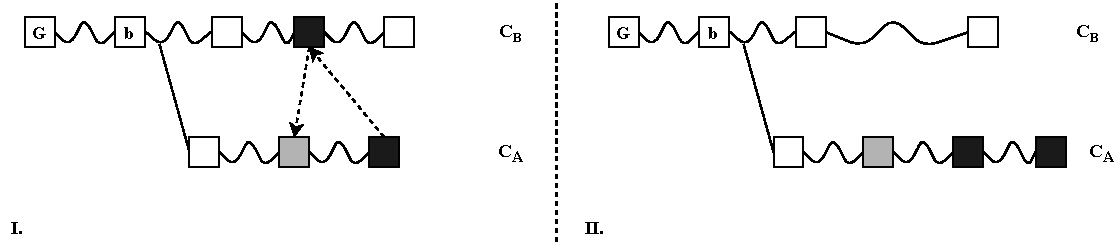
\includegraphics[scale=0.5]{figures/injection.png}
	\end{center}
	\caption{\textit{The adversarial fork chain $C_A$ and chain $C_B$ of an honest
	player. Blocks generated by the adversary are colored black. Dashed arrows
	represent interlink pointers. Wavy lines imply one or more blocks. When an
	adversarially generated block is sewed from $C_B$ into the adversary's suffix
	proof the verifier conceives $C_A$ as longer and $C_B$ as shorter.  \textbf{I:}
	he real picture of the chains. \textbf{II:} Equivalent picture from the verifier's
	perspective considering the hashing power included in the corresponding suffix
	proof of each chain.}}
	\label{fig:injection}
\end{figure}


The protocol patch we suggest can be summarized as follows:\\


\subsubsection*{Protocol Patch for NIPoPows suffix proofs under velvet fork.} In order
to make NIPoPoWs safe under velvet fork conditions we suggest:
\begin{enumerate}
\item Strengthen the Honest Majority Assumption so that $\dfrac{t}{n-t} \leq
\dfrac{1-\delta}{2}$
%%% TODO: also provide short algorithm for the intrlink construction after the patch 
\item The NIPoPoW protocol under velvet fork works as usual but a miner constructs
a block's interlink without pointers to blocks with false interlink except for
pointers of level $\mu = 0$.
\end{enumerate}

Algorithm \ref{alg:updateInterlink} describes the interlink update procedure for the
honest miner after the suggested protocol patch. An honest miner has to first find the
most recent \emph{smooth velvet} and then add pointers so as to consider this block in
the interlink as well. Function \textit{has-correct-interlink(B)} checks whether a
block \textit{B} is a smooth velvet by calling \textit{valid-interlink-pointer(B,p)}
for every pointer \textit{p} in \textit{B}'s interlink. Function
\textit{valid-interlink-pointer(B,p)} returns \emph{true} if $p$ is a valid 
pointer, in essence a pointer to the most recent \emph{smooth velvet}
for the level denoted by the pointer itself. 

\vspace{4mm}

\begin{algorithm}[H]
	%\begin{algorithmic}[1]
		\SetAlgoNoLine
		\DontPrintSemicolon
		\SetKwProg{Fn}{function}{:}{\text{end function}}
		\Fn{updateInterlinkVelvet(C)}{
 			$k \leftarrow 1$\;
 			$B\leftarrow C[-k]$\;
 			\While{has-correct-interlink(B) $=$ false}{
   				$k \leftarrow k + 1$\;
   				$B \leftarrow C[-k]$\;
 			}
 			$B \leftarrow C[-k]$\;
 			interlink$\leftarrow$B.interlink\;
 			\For{$\mu = 0$ to level(B)}{
 				interlink$[\mu]\leftarrow id(B)$
 			}
 			\Return interlink\;
		}
	\vspace{4mm}
	\Fn{has-correct-interlink(B)}{
		\If{B.id $=$ Genesis.id}{
			\Return true\;
		}
 		\For{p $\in$ B.interlink} {
     		\If{valid-interlink-pointer(B, p) $=$ false}{
     			\Return false\;
     		}
 		}
 		\Return true\;
	}

	\vspace{4mm}
	\Fn{valid-interlink-pointer(B, p)}{
		$b \leftarrow Block(B.prevId)$\;
 		\While{b.id $\not =$ p.id} {
     		\If{$ level(b) \geq level(p) \wedge
     			\text{has-correct-interlink(b)} $}{
     			\Return false\;
     		}
     		\If{b.id = Genesis.id}{
     			\Return false\;
     		}
     		$b \leftarrow Block(b.prevId)$
 		}
 		\If{$\text{has-correct-interlink(b)}$}{
 			\Return true\;
 		}
 		\Return false\;
	}
	%\end{algorithmic}
 	\caption{velvet updateInterlink}
 	\label{alg:updateInterlink}
\end{algorithm}

\vspace{4mm}

The following two Lemmas come as immediate results from the suggested protocol update.\\

\textit{\textbf{Lemma 4.} Consider a velvet suffix proof $(\pi, \chi)$ constructed 
by an honest player. The proof subchain $\pi$ cannot contain any block with 
incorrect interlink.}\\

\textit{\textbf{Lemma 5.} Consider $C_B, C_A$ the 0-level chains adopted respectively
by an honest player and the adversary at some round $r'$. Let $\pi_A$ be a velvet
suffix proof constructed by the adversary. If there exist blocks with incorrect
interlinks in $\pi_A$, consider block $b_A$ which was produced at some round
$r_A$ and is the first block in $\pi_A$ that has incorrect interlink. Then
$\forall r: r \geq r_A$ no honest blocks generated at round $r$ can be included in $\pi_A$.} \\

In conclusion the Prove and Verify algorithm for the NIPoPoW suffix protocol remain the same.
